\documentclass[../main.tex]{subfiles}









\begin{document}




\chapter*{Introducció}

Al present capítol trobareu uns apunts detallats d'un curs molt bàsic i introductori sobre topologia. Aquest curs és l'assignatura anomenada ``topologia'', assignatura obligatòria en la carrera de matemàtiques de la Universitat de Barcelona, que jo he cursat aquest 2020. Ara però, el semestre al qual l'he cursada ha estat el semestre de la crisis de la COVID-19, que va obligar a fer les classes online. Així doncs, inicialment aquest curs està basat en els meus apunts de les classes magistrals impartides pel Dr. Ignasi Mundet, així com els problemes impartits pel Dr. Javier Gutiérrez. Ara bé, això va durar escasses setmanes i la veritat és que els professors esmentats van continuar donant-nos bibliografia i exercicis corregits per tal de continuar el curs des de casa.

He de dir, però, que no estic gaire satisfet amb la metodologia proposada pel Mundet, que es va basar en donar tres fonts, i anar actualitzant fins a quin capítol havíem de tenir llegit. Després va començar la iniciativa de fer classes virtuals pel BB Collaborate per resoldre dubtes. A mí em sembla insuficient, però què hi farem. Les fonts donades pel Dr. Mundet són les meves principals fonts per aquest document. Aquestes són \cite{naranjo}, \cite{llerena}, \cite{mathonline}. Els primers són uns apunts bastant antics dels professors J. Naranjo i V. Navarro, que contenen una breu descripció de tots els temes del curs, així com més temes ja que són d'abans del pla Bologna. Els segons són uns apunts de la professora I. Llerena, que consisteixen en una molt més exhaustiva compilació de tot aquest curs, amb molt més material del necessari. Jo només n'he pres una o dues seccions d'aquí, i la resta per complementar (dibuixos, exemples, etc.). La última referència és una pàgina web proporcionada pels professors d'aquesta assignatura que conté un extens curs de topologia. Aquesta ha estat la meva principal font. Tots (o quasi tots) els dibuixos són extrets d'allà i gran part dels exemples també.

D'altra banda, els exercicis (no tots) van ser realitzats pel professor de laboratori, així com també pel Mundet (que a la mateixa vegada era el professor de problemes) i penjats al Campus Virtual seguint la línia cronològica establerta pel pla docent, de forma que la gran majoria d'exercicis realitzats en aquest document provenen directa o semi directament d'aquests exercicis. Altres, però, van ser realitzats del tot per mi, ja que donades les circumstàncies de la COVID-19, es van veure obligats a modificar el mètode d'avaluació i una part consistia en realitzar exercicis i entregar-los cada setmana.

Dit això, també volia agrair l'ajuda d'alguns dels meus companys com el Sixte Oriol Llenas Segura i el Roger Gibert que em van proporcionar apunts i exercicis fets per ells ja que van cursar l'assignatura un any abans que jo, i també a l'Eric Rubia Aguilera, que em va ajudar sempre que li ho vaig demanar i també em va proporcionar exercicis corregits i esclariments teòrics.

Per últim, volia afegir que aquest és un document que conté bàsicament apunts. No té cap intenció d'ésser un treball ben presentat ni res de l'estil, amb la qual cosa és bastant possible que hi hagi faltes o errors tipogràfics que se m'hagin passat ja que no ho he revisat com si fos un treball a avaluar, perquè no ho és. Si es detecten errors greus seria d'agrair que se m'avisés.

\subfile{chapters/espais_metrics.tex}
\subfile{chapters/espais_topologics.tex}
\subfile{chapters/oberts_i_tancats.tex}
\subfile{chapters/bases_de_topologies.tex}
\subfile{chapters/aplicacions_continues.tex}
\subfile{chapters/construccio.tex}
\subfile{chapters/separacio.tex}
\subfile{chapters/compacitat.tex}
\subfile{chapters/connexio.tex}


\chapter{Appèndix: Projecció estereogràfica}















\section{En dimensió 1}

Aquesta és una aplicació que serveix com a exemple d'homeomorfisme entre l'espai topològic $S^1\setminus\{(0,1)\}$ i l'espai topològic $\mathbb{R}$, amb la topologia euclidiana. Dir que $S^1\setminus\{(0,1)\}\cong \mathbb{R}$ seria com dir que si agafem la recta real $\mathbb{R}$ dels ``extrems'' i els ajuntem en un punt (inexistent, ja que aquests extrems són inexistents) obtenim un espai amb les mateixes característiques.

Més tard, veiem que si omplim aquest punt inexistent, que és el $(0,1)$ (encara que serveix qualsevol altre punt que no sigui $(\pm 1,0)$) aleshores obtenim la compactificació d'Alexandroff de l'espai $\mathbb{R}$.
\subsection{Interpretació gràfica}

La projecció estereogràfica és una funció que agafa un punt $p$ de la circumferència $S^1$, tret del $(0,1)$ i l'envia a un altre punt de la recta $\mathbb{R}$, que correspon al punt intersecció de la recta $\overline{(0,1)p}$ amb l'eix de les abscisses.

\begin{equation}
    \notag
    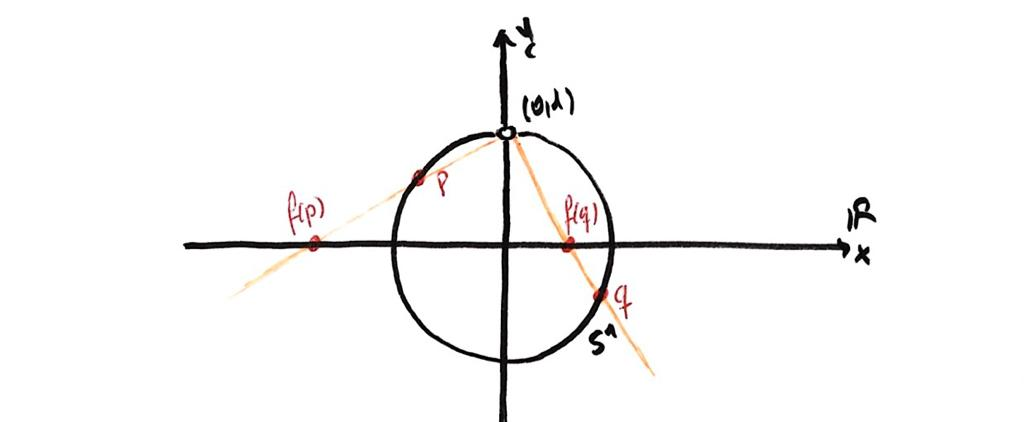
\includegraphics[scale = 0.3]{fotos_topo_1/projeccioestereografica.jpeg}
\end{equation}

\subsection{Construcció de la funció explícita}

$p = (\alpha,\beta)\in S^1\setminus\{(0,1)\}$, és a dir, que satisfà $\alpha^2 + \beta^2 = 1$, i $\alpha\not=0$, $\beta\not=1$. Aleshores construeixo la recta de $(\alpha,\beta)$ a $(0,1)$. El vector director serà $(\alpha,\beta-1)$. Així doncs, $r:(1-\beta)x+\alpha y+C = 0$ i imposant que passa pel punt $(0,1)$ obtenim $\alpha =C\Rightarrow C = -\alpha$. Aleshores tenim la recta
\begin{equation}
    \notag
    r: (1-\beta)x + \alpha y - \alpha = 0
\end{equation}
La intersequem amb l'eix de les $x$ que té com a equació $y = 0$ i obtenim
\begin{equation}
    \notag
    (1-\beta)x-\alpha = 0\Longrightarrow x = \frac{\alpha}{1-\beta}
\end{equation}
Per tant, la projecció estereogràfica és la funció 
\begin{equation}
    \notag
    \begin{array}{rl}
        f:S^1\setminus\{(0,1)\} & \longrightarrow\mathbb{R} \\
        (x,y) & \longmapsto \dfrac{x}{1-y}
    \end{array}
\end{equation}

\subsection{Demostrem que és un homeomorfisme}
Veiem que aquesta $f$ és un homeomorfisme. 
\begin{enumerate}[(i)]
    \item Clarament és una funció contínua, ja que $y\not=0$ perquè estem prenent els punts de $S^1\setminus\{(0,1)\}$.
    \item Veiem que sigui bijectiva. 
\end{enumerate}


\section{En dimensió 2}
\begin{equation}
    \notag
    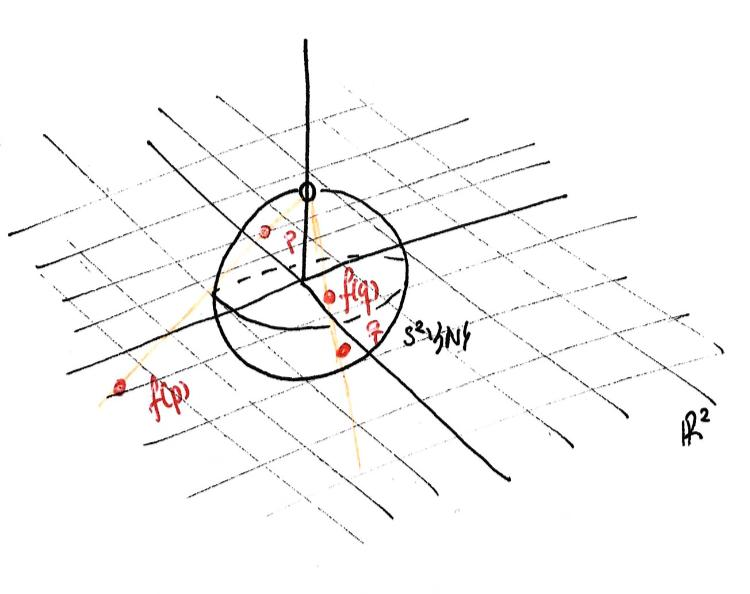
\includegraphics[scale = 0.3]{fotos_topo_1/projeccioestereografica2.jpeg}
\end{equation}

Per veure-ho en dimensió 2 accedir a \cite{bestiariotopologico}






\end{document}